\subsection{Übung 2: Generator}

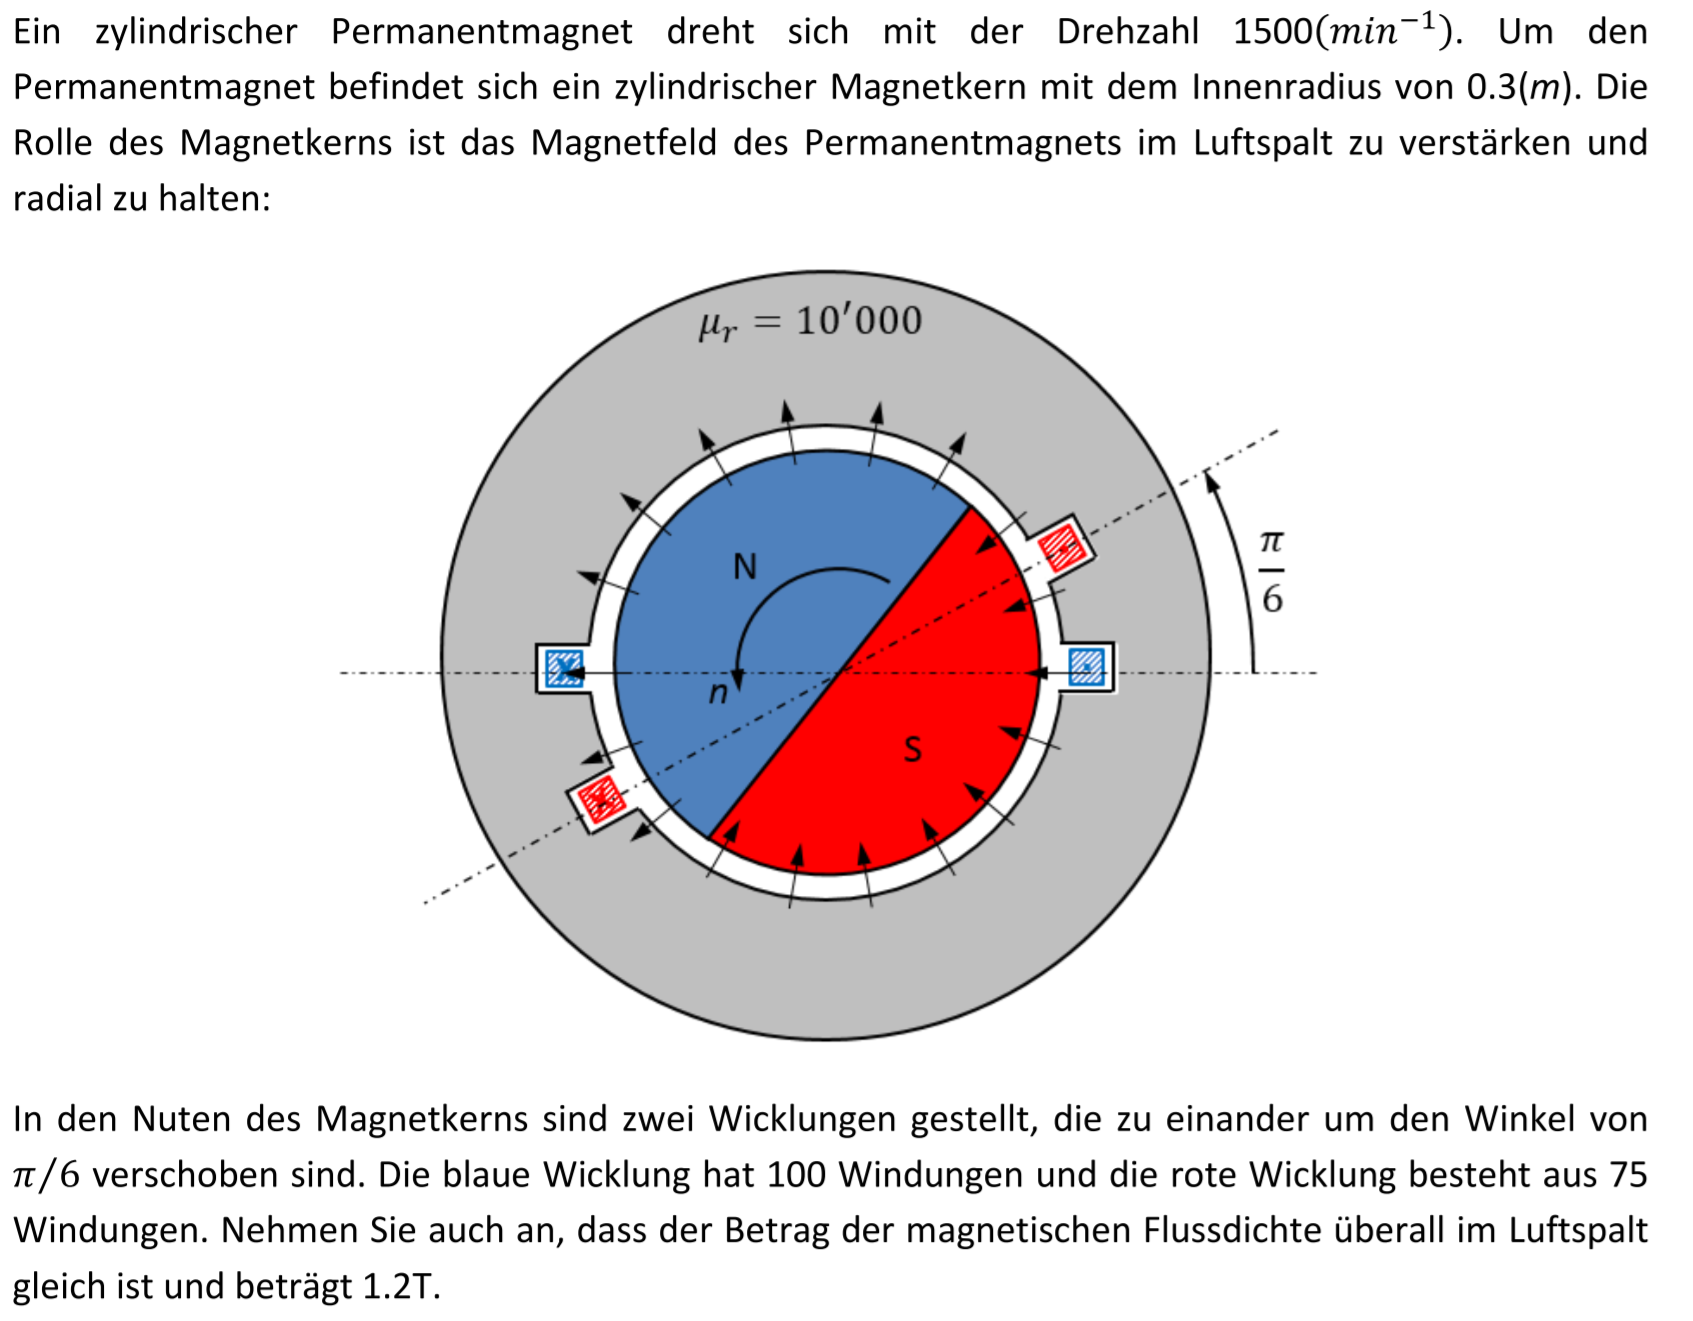
\includegraphics[width = 0.8\textwidth]{bilder/a21.png}

Um den magnetischen Fluss darstellen zu können muss man sich vorstellen dass der Fluss um die Spule fliessen muss, was bei einer konstanten Flussdichte direkt von der Fläche abhängig ist.
\begin{align*}
	\Phi_{blau}(\alpha) &= B \cdot r\cdot  l \cdot (\pi - \alpha) -  B\cdot r\cdot l\cdot \alpha = B \cdot r\cdot  l \cdot (\pi - 2\cdot \alpha) &(0\leq \alpha \leq \pi)\\
	\Phi_{blau}(\alpha) &=  -B \cdot r\cdot  l \cdot (3\pi - 2\cdot \alpha) &(\pi\leq \alpha \leq 2\pi)\\
	\Phi_{rot}(\alpha) &= B \cdot r\cdot  l \cdot (\pi - 2\cdot \alpha+\frac{\pi}{3}) &(\frac{\pi}{6}\leq \alpha \leq \frac{7\pi}{6})\\
	\Phi_{rot}(\alpha) &= -B \cdot r\cdot  l \cdot (3\pi - 2\cdot \alpha+\frac{\pi}{3}) &(\frac{7\pi}{6}\leq \alpha \leq \frac{13\pi}{6})
\end{align*}
	
Die induzierte Spannung ist nun $u(t) = L\dfrac{di(t)}{dt} = -N\dfrac{d\Phi}{dt}$

\begin{align*}
	u_{blau}(t) &= -N\frac{d\Phi}{dt} = -N\cdot B \cdot r  \cdot l\cdot \left(\pi - \frac{2 \pi\cdot n \cdot t}{60} \right) \frac{1}{dt}\qquad = N\cdot B \cdot r\cdot l \cdot \pi \frac{n}{15} &(0\leq \alpha \leq \pi)\\
	u_{blau}(t) &= -N\frac{d\Phi}{dt} = N\cdot B \cdot r  \cdot l\cdot \left(\pi - \frac{2 \pi\cdot n \cdot t}{60} \right) \frac{1}{dt}\qquad = -N\cdot B \cdot r\cdot l \cdot \pi \frac{n}{15} &(\pi\leq \alpha \leq 2\pi)\\
\end{align*}
Die Spannung für die rote Spule wird gleich berechnet, einfach erneut um $\frac{\pi}{6}$ Phasenverschoben.

